\section{A case study of \OpenCL optimizations}
\label{sec:reduce:case-study}
To understand the problems of performance and portability in the context of modern parallel processors we will study a simple application example: parallel reduction.
This discussed is based on the presentation \emph{``Optimizing Parallel Reduction in CUDA''} by \citeauthor{Harris2007}~\cite{Harris2007} where optimizations for implementing parallel reduction using \CUDA and targeting Nvidia \GPUs are presented.
Optimization guidelines like this exist from every hardware vendor giving application developers advice on how to exploit their hardware~\cite{CUDAProgrammingGuide,AMDProgrammingGuide,IntelGPUProgrammingGuide,IntelXeonProgrammingGuide}.

In \autoref{chapter:skelcl} we saw that we can express a parallel reduction using a single algorithmic skeleton: \reduce.
Here we look at how efficient \OpenCL implementation of this algorithm look like.
We are especially interested in gradually optimizing this application to see how beneficial the single optimization steps are.

We will first start by looking at the implementation and optimizations on one particular hardware architecture, using Nvidia's Fermi \GPU architecture as our example.
Then we will see how the optimized implementations perform on an AMD \GPU and Intel \CPU, to evaluate their portability.
Finally, we will use our observations to motivate the need for a pattern-based code generator for achieving performance portability.


\subsection{Optimizing parallel reduction for Nvidia's \GPU architectures}
For implementing the parallel reduction, or more precisely the parallel summation of an array, an approach using two \OpenCL kernels is used.
The first \OpenCL kernel is executed in parallel by multiple \OpenCL work-groups, each producing a temporary result, then the second \OpenCL kernel is executed by a single \OpenCL work-group producing the final result.
This strategy is applied as global synchronization, \ie, synchronization across work-groups, is prohibited in \OpenCL.
By using the two kernel approach massive parallelism can be exploited in the first phase as multiple work-groups operate concurrently on independent parts of the input array.
The synchronization inside the second work-group ensures correctness when computing the final result.

We will follow the methodology in~\cite{Harris2007} and evaluate the performance of the different versions using the measured memory bandwidth as our metric.
This is reasonable as the reduction has a very low arithmetic intensity and its performance is, therefore, bound by the available memory bandwidth.

\paragraph{First \OpenCL implementation}
\autoref{lst:reduce0} shows the first, basic version of the parallel reduction in \OpenCL.
This will be our starting point for the following optimizations.
In this implementation each work-item first loads an element into the local memory (line~\ref{lst:reduce0:load}).
After a synchronization (line~\ref{lst:reduce0:firstBarrier}) all work-items of a work-group execute a for loop (lines~\ref{lst:reduce0:for:start}--\ref{lst:reduce0:for:end}) to perform a collective tree-based reduction.
In every iteration the if statement (line~\ref{lst:reduce0:if}) ensures that a declining number of work-items remain active performing partial reductions in the shrinking reduction tree.
The second barrier in line~\ref{lst:reduce0:for:end} ensures that no race conditions occurs when accessing the shared local memory.
Finally, the work-item in the work-group with id zero writes back the computed result to the global memory in line~\ref{lst:reduce0:writeBack}.

The implementation presented in \autoref{lst:reduce0} is not straightforward to implement.
The application developer has to be familiar with the parallel execution model of \OpenCL to avoid race conditions and deadlocks.
For example, it is important that the second barrier in line~\ref{lst:reduce0:for:end} is placed \emph{after} and not \emph{inside} the if statement.
This is true, even though, work-items not entering the if statement will never read from or write to memory and, therefore, can never be influenced by a race condition.
Nevertheless, \OpenCL requires all work-item from a work-group to execute all barrier statements in a kernel exactly the same number of times.
The application developer is responsible to ensure that this condition is met, otherwise a deadlock will occur.

Putting the programming difficulties aside this implementation does not provide high performance.
\citeauthor{Harris2007} reports that only 2.41\% of the theoretical peak memory bandwidth are utilized. 

\begin{lstlisting}[%                                                             
caption={First \OpenCL implementation of the parallel reduction achieving 2.41\% of the theoretical peak memory bandwith performance.},%
numbers=left,%
float=tb,
label={lst:reduce0}]
kernel
void reduce0(global float* g_idata, global float* g_odata,
             unsigned int n, local float* l_data) {
  unsigned int tid = get_local_id(0);
  unsigned int i   = get_global_id(0);
  l_data[tid] = (i < n) ? g_idata[i] : 0;$\label{lst:reduce0:load}$
  barrier(CLK_LOCAL_MEM_FENCE);$\label{lst:reduce0:firstBarrier}$

  // do reduction in local memory
  for(unsigned int s=1; s < get_local_size(0); s *= 2) {$\label{lst:reduce0:for:start}$
    if ((tid % (2*s)) == 0) {$\label{lst:reduce0:if}$
      l_data[tid] += l_data[tid + s]; }
    barrier(CLK_LOCAL_MEM_FENCE); }$\label{lst:reduce0:for:end}$

  // write result for this work-group to global memory
  if (tid == 0) g_odata[get_group_id(0)] = l_data[0]; }$\label{lst:reduce0:writeBack}$
\end{lstlisting}

\FloatBarrier
\newpage

\paragraph{Avoid divergent branching}

\autoref{lst:reduce1} shows the second implementation.
The differences from the previous implementation are highlighted in the code.

When performing the collective tree-based reduction in a work-group a shrinking number of work-items remains active until the last remaining work-item computes the result of the entire work-group.
In the previous version the modulo operator was used to determine which work-item remains active (see line~\ref{lst:reduce0:if} in \autoref{lst:reduce0}).
This leads to a situation were not consecutive work-items remain active, but work-items which id is divisible by 2, then by 4, then by 8, and so on.
In Nvidia's \GPU architectures 32 work-items are grouped into a \emph{warps} and executed together, as described in \autoref{chapter:background}.
It is highly beneficial to program in a style where all 32 work-items of a warp perform the same instructions, especially, to avoid divergent branching between work-items of a warp.
Using the modulo operator to determine the active work-items leads to highly divergent branching.
The second implementation in \autoref{lst:reduce1}, therefore, uses a different formula (line~\ref{lst:reduce1:index}) to determine the active work-items which avoids divergent branching.

The performance improves by a factor of 2.33 as compared to the first implementation.
Still only 5.62\% of the theoretically available memory bandwidth are used by this version.

\begin{lstlisting}[%                                                             
caption={\OpenCL implementation of the parallel reduction avoiding divergent branching.
         This implementation achieves 5.62\% of the theoretical peak memory bandwidth performance.},%
numbers=left,%
float=tb,
label={lst:reduce1}]
kernel
void reduce1(global float* g_idata, global float* g_odata,
             unsigned int n, local float* l_data) {
  unsigned int tid = get_local_id(0);
  unsigned int i   = get_global_id(0);
  l_data[tid] = (i < n) ? g_idata[i] : 0;
  barrier(CLK_LOCAL_MEM_FENCE);

  for(unsigned int s=1; s < get_local_size(0); s *= 2) {
      // continuous work-items remain active
      $\strut$@int index = 2 * s * tid;@$\label{lst:reduce1:index}$
      if (@index < get_local_size(0)@) {$\label{lst:reduce1:if}$
          l_data[index] += l_data[index + s]; }$\label{lst:reduce1:read}$
      barrier(CLK_LOCAL_MEM_FENCE); }

  if (tid == 0) g_odata[get_group_id(0)] = l_data[0]; }
\end{lstlisting}


\paragraph{Avoid interleaved addressing}

\autoref{lst:reduce2} shows the third implementation.
The differences from the previous implementation are highlighted in the code.

On modern \GPUs the fast local memory is organized in multiple \emph{banks}.
When two, or more, work-items simultaneously access memory locations in the same bank a \emph{bank conflict} occurs which means that all memory requests are answered sequentially and not in parallel as usual.
This is described in more detail in~\autoref{chapter:background}.
The previous two implementation use an access pattern for the local memory which makes bank conflicts likely.
When reading memory from the local memory in line~\ref{lst:reduce1:read} of \autoref{lst:reduce1} each work-item reads interleaved from two locations: \lstinline!index! and \lstinline!index+s!.
The third implementation in \autoref{lst:reduce2} avoids this problematic local memory access pattern.
Instead a sequential access pattern is used where consecutive work-items access consecutive memory locations.
This is achieved by directly using the local id as index together with a different definition of \lstinline!s! in line~\ref{lst:reduce2:s}.
This better access pattern requires the reduction operation to be commutative, as the order of element is not respected when reading from global memory.

The performance improves by a factor of 2.01 as compared to the previous implementation and 4.68 to the initial implementation.
With this version 11.27\% of the theoretically available memory bandwidth are used.


\begin{lstlisting}[%                                                             
caption={\OpenCL implementation of the parallel reduction avoiding local memory bank conflicts.
         This implementation achieves 11.27\% of the theoretical peak memory bandwidth performance.},%
numbers=left,%
float=tb,
label={lst:reduce2}]
kernel
void reduce2(global float* g_idata, global float* g_odata,
             unsigned int n, local float* l_data) {
  unsigned int tid = get_local_id(0);
  unsigned int i   = get_global_id(0);
  l_data[tid] = (i < n) ? g_idata[i] : 0;
  barrier(CLK_LOCAL_MEM_FENCE);

  // process elements in different order
  // requires commutativity!
  for(@unsigned int s=get_local_size(0)/2; s>0; s>>=1@) {$\label{lst:reduce2:s}$
      if (@tid < s@) {
          l_data[@tid@] += l_data[@tid@ + s]; }
      barrier(CLK_LOCAL_MEM_FENCE); }

  if (tid == 0) g_odata[get_group_id(0)] = l_data[0]; }
\end{lstlisting}

\paragraph{Increase computational intensity per work-item}

\autoref{lst:reduce3} shows the fourth implementation.
The differences from the previous implementation are highlighted in the code.

For the previous versions each work-item loads one element from global into local memory before the work-group collectively performs a tree-based reduction.
That means that half of the work-items are idle after performing a single copy operation, which is highly wasteful.
The fourth implementation in \autoref{lst:reduce3} avoids this by letting each work-item load two elements from global memory, perform an addition, and store the computed result in local memory.
Assuming the same input size this reduces the number of work-items to start by half and, therefore, increases the computational intensity for every work-item.

The performance improves by a factor of 1.78 as compared to the previous implementation and 8.34 to the initial implementation.
With this version 20.11\% of the theoretically available memory bandwidth are used.


\begin{lstlisting}[%                                                             
caption={\OpenCL implementation of the parallel reduction. Each work-item performs an addition when loading data from global memory.
         This implementation achieves 20.11\% of the theoretical peak memory bandwidth performance.},%
numbers=left,%
float=tb,
escapechar=\`,
label={lst:reduce3}]
kernel
void reduce3(global float* g_idata, global float* g_odata,
             unsigned int n, local float* l_data) {
  unsigned int tid = get_local_id(0);
  $\strut$@unsigned int i = get_group_id(0) * (get_local_size(0)*2)@
                                   $\strut$@+ get_local_id(0);@
  l_data[tid] = (i < n) ? g_idata[i] : 0;
  // performs first addition during loading
  $\strut$@if (i + get_local_size(0) < n)@
  $\strut$@    l_data[tid] += g_idata[i+get_local_size(0)];@
  barrier(CLK_LOCAL_MEM_FENCE);

  for(unsigned int s=get_local_size(0)/2; s>0; s>>=1) {
      if (tid < s) {
          l_data[tid] += l_data[tid + s]; }
      barrier(CLK_LOCAL_MEM_FENCE); }

  if (tid == 0) g_odata[get_group_id(0)] = l_data[0]; }
\end{lstlisting}

\newpage

\paragraph{Avoid synchronization inside a warp}

\autoref{lst:reduce4} shows the fifth implementation.
The differences from the previous implementation are highlighted in the code.

Wraps are the fundamental execution unit in Nvidia's \GPU architectures, as explained in \autoref{chapter:background}.
32 work-items are grouped together to form a warp based on their id, \ie, work-items with id 0 -- 31 are grouped into the first warp, work-items with id 32 -- 63 into the second warp, \etc.
All work-items grouped in a warp are guaranteed to be executed together in a lock-step manner:
all work-items in the same warp execute the same instruction simultaneously.
Because of this hardware behaviour, no barrier synchronization is required between instructions inside a single warp.
The fifth implementation in \autoref{lst:reduce4} takes advantage of this.
The for loop performing the tree-based reduction is left early at the stage when only 32 work-items remain active (see line~\ref{lst:reduce4:for}).
Lines~\ref{lst:reduce4:warp:start}--\ref{lst:reduce4:warp:end} shows the special code which performs the rest of the tree-base reduction without any barrier synchronization.
The code shown here effectively unrolled the last six iterations of the for loop in line~\ref{lst:reduce4:for}.
As warps are specific to Nvidias \GPU architectures, this implementation is not portable \OpenCL code and will produce incorrect results on other \OpenCL devices.

The performance improves by a factor of 1.8 as compared to the previous implementation and 15.01 to the initial implementation.
With this version 36.21\% of the theoretically available memory bandwidth are used.

\begin{lstlisting}[%                                                             
caption={\OpenCL implementation of the parallel reduction.
         Synchronization inside a warp is avoided by unrolling the loop for the last 32 work-items.
         This implementation achieves 36.21\% of the theoretical peak memory bandwidth performance.},%
numbers=left,%
float=p,
label={lst:reduce4}]
kernel
void reduce4(global float* g_idata, global float* g_odata,
             unsigned int n,local volatile float* l_data){
  unsigned int tid = get_local_id(0);
  unsigned int i = get_group_id(0) * (get_local_size(0)*2)
                                   + get_local_id(0);
  l_data[tid] = (i < n) ? g_idata[i] : 0;
  if (i + get_local_size(0) < n) 
      l_data[tid] += g_idata[i+get_local_size(0)];  
  barrier(CLK_LOCAL_MEM_FENCE);

  // prevent further unrolling (see next version)
  $\strut$@#pragma unroll 1@$\label{lst:reduce4:pragma}$
  for(unsigned int s=get_local_size(0)/2; s>@32@; s>>=1) {$\label{lst:reduce4:for}$
      if (tid < s) {
          l_data[tid] += l_data[tid + s]; }
      barrier(CLK_LOCAL_MEM_FENCE); }

  // unroll for last 32 active work-items
  // no synchronization required on NVIDIA GPUs
  // this is not protable OpenCL code!
  $\strut$@if (tid < 32) {@$\label{lst:reduce4:warp:start}$
  $\strut$@  if (WG_SIZE >= 64) { l_data[tid] += l_data[tid+32]; }@
  $\strut$@  if (WG_SIZE >= 32) { l_data[tid] += l_data[tid+16]; }@
  $\strut$@  if (WG_SIZE >= 16) { l_data[tid] += l_data[tid+ 8]; }@
  $\strut$@  if (WG_SIZE >=  8) { l_data[tid] += l_data[tid+ 4]; }@
  $\strut$@  if (WG_SIZE >=  4) { l_data[tid] += l_data[tid+ 2]; }@
  $\strut$@  if (WG_SIZE >=  2) { l_data[tid] += l_data[tid+ 1]; }@
  $\strut$@}@$\label{lst:reduce4:warp:end}$

  if (tid == 0) g_odata[get_group_id(0)] = l_data[0]; }
\end{lstlisting}

\paragraph{Complete loop unrolling}

\autoref{lst:reduce5} shows the sixth implementation.
The differences from the previous implementation are highlighted in the code.

In the previous implementation we made a special case for the last six iterations of the for loop and provided special code handling each iteration separately.
This is a general optimization strategy known as \emph{loop unrolling}.
Loop unrolling can be beneficial because variables and branches required by the loop can be avoided.
In the sixth implementation shown in \autoref{lst:reduce5} the for loop has been removed entirely and the replaced by three if statement (line~\ref{lst:reduce5:if:1},~\ref{lst:reduce5:if:2}, and~\ref{lst:reduce5:if:3}).
Each if statement replaces one iteration of the loop.
This code assumes that \code{WG\_SIZE} is a compile time constant and, therefore, the if statements will be evaluated at compile time, avoiding costly branches at runtime.
Different to the previous optimization we still have to provide a barrier to ensure correct synchronization, as multiple warps are involved here.

The performance improves by a factor of 1.41 as compared to the previous implementation and 21.16 to the initial implementation.
With this version 56.92\% of the theoretically available memory bandwidth are used.

\begin{lstlisting}[%                                                             
caption={\OpenCL implementation of the parallel reduction with a completly unrolled loop.
         This implementation achieves 56.92\% of the theoretical peak memory bandwidth performance.},%
numbers=left,%
float=p,
label={lst:reduce5}]
kernel
void reduce5(global float* g_idata, global float* g_odata,
             unsigned int n,local volatile float* l_data){
  unsigned int tid = get_local_id(0);
  unsigned int i = get_group_id(0) * (get_local_size(0)*2)
                                   + get_local_id(0);
  l_data[tid] = (i < n) ? g_idata[i] : 0;
  if (i + get_local_size(0) < n) 
      l_data[tid] += g_idata[i+get_local_size(0)];  
  barrier(CLK_LOCAL_MEM_FENCE);

  // unroll for loop entirely
  $\strut$@if (WG_SIZE >= 512) {@$\label{lst:reduce5:if:1}$
  $\strut$@    if (tid < 256) { l_data[tid] += l_data[tid+256]; }@
  $\strut$@    barrier(CLK_LOCAL_MEM_FENCE); }@
  $\strut$@if (WG_SIZE >= 256) {@$\label{lst:reduce5:if:2}$
  $\strut$@    if (tid < 128) { l_data[tid] += l_data[tid+128]; }@
  $\strut$@    barrier(CLK_LOCAL_MEM_FENCE); }@
  $\strut$@if (WG_SIZE >= 128) {@$\label{lst:reduce5:if:3}$
  $\strut$@    if (tid <  64) { l_data[tid] += l_data[tid+ 64]; }@
  $\strut$@    barrier(CLK_LOCAL_MEM_FENCE); }@
  
  if (tid < 32) {
    if (WG_SIZE >= 64) { l_data[tid] += l_data[tid+32]; }
    if (WG_SIZE >= 32) { l_data[tid] += l_data[tid+16]; }
    if (WG_SIZE >= 16) { l_data[tid] += l_data[tid+ 8]; }
    if (WG_SIZE >=  8) { l_data[tid] += l_data[tid+ 4]; }
    if (WG_SIZE >=  4) { l_data[tid] += l_data[tid+ 2]; }
    if (WG_SIZE >=  2) { l_data[tid] += l_data[tid+ 1]; } }
  
  if (tid == 0) g_odata[get_group_id(0)] = l_data[0]; }
\end{lstlisting}


\paragraph{Fully optimized implementation}

\autoref{lst:reduce6} shows the last and fully optimized implementation.
The differences from the previous implementation are highlighted in the code.

One of the optimizations applied earlier was to increase the computational intensity for each single work-item by performing two loads and an addition instead of a single load.
This final version applies the same idea, but performing multiple additions per work-item before the collective tree-based reduction with the entire work-group.
This has indeed two advantages:
first, the algorithmic intensity is increased, \ie, each work-item is doing more work,
and, second, performing the summation sequentially by a single work-item does not require costly synchronizations.
The fully optimized implementation is shown in \autoref{lst:reduce6} with the changes highlighted.
A while loop has been introduced (see line~\ref{lst:reduce6:while}) which, in every iteration, loads two elements from global memory and adds them to the local memory.
No synchronization is required here as each work-item operates independently on different memory locations.
The way the memory is accessed ensures that memory accesses will be coalesced when reading from global memory.

The performance improves by a factor of 1.42 as compared to the previous implementation and 30.04 to the initial implementation.
With this version 72.53\% of the theoretically available memory bandwidth are used.

\begin{lstlisting}[%                                                             
caption={Fully optimized \OpenCL implementation of the parallel reduction.
         This implementation achieves 72.53\% of the theoretical peak memory bandwidth performance.},%
numbers=left,%
float=p,
label={lst:reduce6}]
kernel
void reduce6(global float* g_idata, global float* g_odata,
             unsigned int n,local volatile float* l_data){
  unsigned int tid = get_local_id(0);
  unsigned int i = get_group_id(0) * (get_local_size(0)*2)
                                   + get_local_id(0);
  $\strut$@unsigned int gridSize = WG_SIZE*2*get_num_groups(0);@
  $\strut$@l_data[tid] = 0;@

  // multiple elements are reduced per work-item
  $\strut$@while (i < n) { l_data[tid] += g_idata[i];@$\label{lst:reduce6:while}$
  $\strut$@                if (i + WG_SIZE < n)@
  $\strut$@                  l_data[tid] += g_idata[i+WG_SIZE];@
  $\strut$@                i += gridSize; }@
  barrier(CLK_LOCAL_MEM_FENCE);

  if (WG_SIZE >= 512) {
      if (tid < 256) { l_data[tid] += l_data[tid+256]; }
      barrier(CLK_LOCAL_MEM_FENCE); }
  if (WG_SIZE >= 256) {
      if (tid < 128) { l_data[tid] += l_data[tid+128]; }
      barrier(CLK_LOCAL_MEM_FENCE); }
  if (WG_SIZE >= 128) {
      if (tid <  64) { l_data[tid] += l_data[tid+ 64]; }
      barrier(CLK_LOCAL_MEM_FENCE); }
  
  if (tid < 32) {
    if (WG_SIZE >= 64) { l_data[tid] += l_data[tid+32]; }
    if (WG_SIZE >= 32) { l_data[tid] += l_data[tid+16]; }
    if (WG_SIZE >= 16) { l_data[tid] += l_data[tid+ 8]; }
    if (WG_SIZE >=  8) { l_data[tid] += l_data[tid+ 4]; }
    if (WG_SIZE >=  4) { l_data[tid] += l_data[tid+ 2]; }
    if (WG_SIZE >=  2) { l_data[tid] += l_data[tid+ 1]; } }
  
  if (tid == 0) g_odata[get_group_id(0)] = l_data[0]; }
\end{lstlisting}


\paragraph{Conclusions}
We can draw valuable conclusions from studying these \OpenCL source codes.

The first conclusion is, that implementing these optimizations is not intuitive and straightforward.
It requires experience as well as knowledge and reasoning about the target hardware architecture, in this case Nvidia's Fermi \GPU architecture:
\autoref{lst:reduce1} requires the understanding of the problem of \emph{branch divergence}, \autoref{lst:reduce2} requires knowledge about the organization of local memory and \emph{bank conflicts}, \autoref{lst:reduce3} and \autoref{lst:reduce6} require reasoning about the \emph{computational intensity} of work-items, \autoref{lst:reduce4} requires understanding of \emph{warps} and their execution by the hardware, \autoref{lst:reduce5} requires experience with \emph{loop unrolling} techniques, and, finally, \autoref{lst:reduce6} required knowledge about the organization of global memory and \emph{memory coalescing}.
The author wants to empathize that these are \emph{additional} burdens for the application developer on top of implementing a functionally correct version facing widely recognized problems of parallel programming like dealing with race conditions and deadlocks.

The second conclusion we can draw is, that performing these optimizations on modern parallel architectures is highly beneficial.
The first unoptimized version did only utilize about 2.5\% of the available memory bandwidth, while the fully optimized version utilizes a more reasonable 72.53\%.
Applying all optimizations improved the performance by a factor of $30$ while utilizing the exact same hardware.
Modern parallel processors are often chosen as target architecture because of their high theoretical performance.
Turning the theoretical performance into practical performance by applying these optimizations is, therefore, \emph{essential} for most users.





\subsection{Portability of the optimized parallel reduction}
After we have established how crucial but hard to achieve optimizations are, we now will investigate their portability.
To do so, we run the code shown in \autoref{lst:reduce0}--\ref{lst:reduce6} on three different hardware architectures:
Nvidia's Fermi \GPU architecture~\cite{} which we have used in our analysis in the last section, AMD's Tahiti \GPU architecture~\cite{}, and Intel's Nehalem \CPU architecture~\cite{}.
\autoref{fig:reduce:overview} shows the performance numbers for each architecture.
We use, as before, the memory bandwidth as our performance metric and show the hardware memory bandwidth limit of each respective hardware architecture.
As a practical comparison we also show performance numbers for the parallel reduction using highly tuned, architecture specific implementations of the BLAS library.
We use the cuBLAS library~\cite{} for the Nvidia \GPU, the clBLAS library~\cite{} for the AMD \GPU, and the MKL library~\cite{} for the Intel \CPU.
Each of these libraries is implementation and provided by the corresponding hardware vendor.

\begin{figure}[p]
  \centering
\begin{subfigure}{\linewidth}
  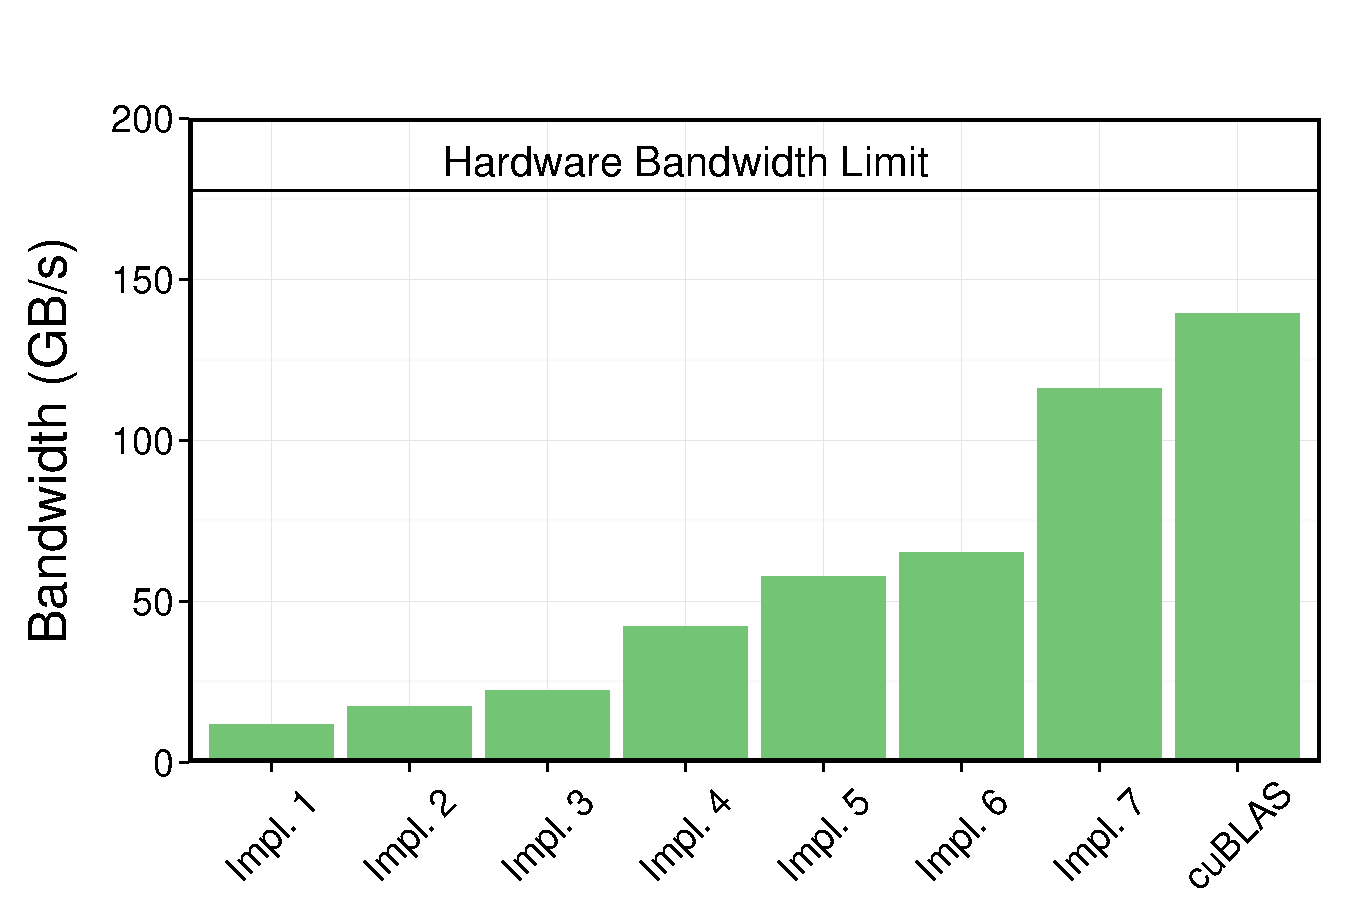
\includegraphics[width=.85\linewidth]{Plots/Reduction/reduce_nv}
  \caption{Nvidia's GTX 480 \GPU.}
  \label{fig:reduce:nvidia}
\end{subfigure}\\
\begin{subfigure}{\linewidth}
  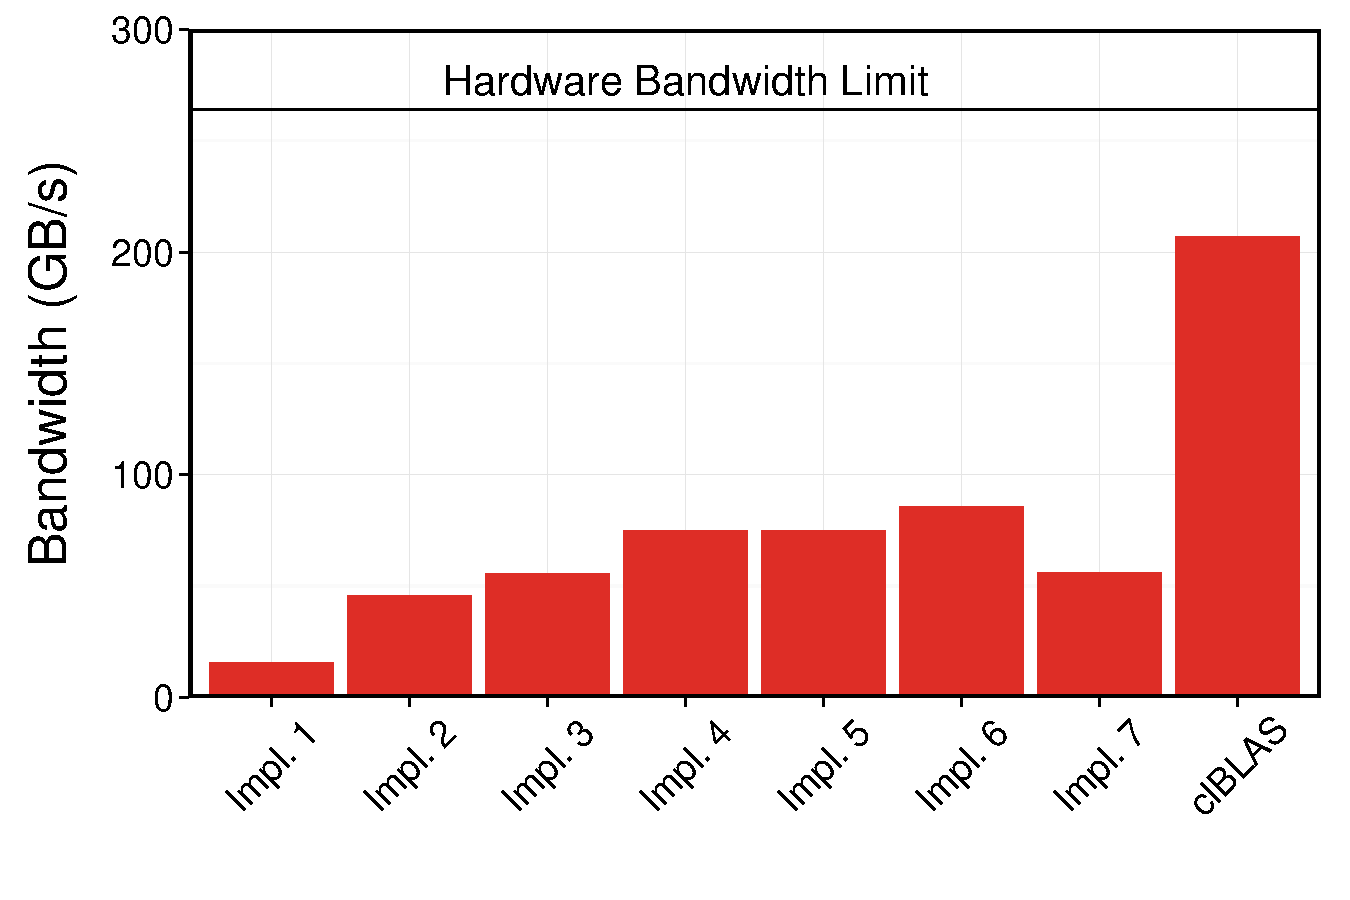
\includegraphics[width=.85\linewidth]{Plots/Reduction/reduce_amd}
  \caption{AMD's HD 7970 \GPU.}
  \label{fig:reduce:amd}
\end{subfigure}\\
\begin{subfigure}{\linewidth}
  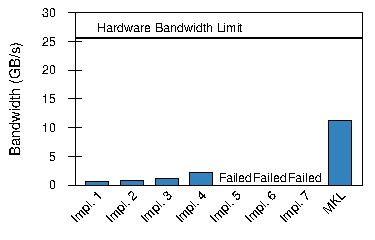
\includegraphics[width=.85\linewidth]{Plots/Reduction/reduce_intel}
    \caption{Dual-socket machine using Intel's E5530 \CPU.}
  \label{fig:reduce:intel}
\end{subfigure}
  \caption{Performance of differently optimized implementations of the parallel reduction.}
  \label{fig:reduce:overview}
\end{figure}


\paragraph{Portability of Optimizations}
The results show that the optimizations discussed in the previous section are not portable. 
On each architecture a different of the optimized implementations performs best:
Implementation~7 (shown in \autoref{lst:reduce6}) on the Nvidia \GPU, Implementation~6 (shown in \autoref{lst:reduce5}) on the AMD \GPU, and Implementation~4 (shown in \autoref{lst:reduce3}) on the Intel \CPU.
Some implementations actually produce incorrect results on the Intel \CPU due to the warp specific optimization introduced in Implementation~5 (shown in \autoref{lst:reduce4}).
Interestingly this optimization happens to be valid on AMD's \GPU architecture as well, as there exists a similar concept to warps called \emph{wavefronts}~\cite{}.

\paragraph{Portability of Relative Performance}
The achieved \emph{relative performance} differs widely across architectures as well.
\emph{Relative performance} refers to the performance of an implementation relative to the best theoretical or practical performance possible on the same hardware architecture.
The theoretical performance of an architecture is given by its hardware limitations, like the number of arithmetic logical units, the width of the memory bus, or the maximum clock frequency.
Practical issues like work load and utilization or the cache miss rate are ignored.
Possible metrics for measuring the theoretical performance are number of floating point operation in GFLOP/s or the memory bandwidth in GB/s.

The best practical performance can be measured by comparison with the best possible implementation available for a particular hardware platform.
It is, obviously, not always possible to determine which implementation is the best.
Here we consider library implementations tuned by the respective hardware vendors as the best available.

By looking at the relative performance we can compare how well optimizations apply across different hardware architectures.

On the Nvidia \GPU the best optimized implementation achieves 83.3\% of the performance of the vendor provided cuBLAS implementation and utilizes 65.4\% of the theoretical peak memory bandwidth.

On the AMD \GPU the gap between the manual and library implementation is much larger:
the manually optimized implementation achieves only 41.3\% of the clBLAS library implementation.
Only 32.4\% of the theoretical peak memory bandwidth is achieved.

On the Intel \CPU Implementation~4 achieves just 16.6\% of the MKL performance.
That means, that MKL is over 5 times faster than the best of the presented optimized implementations.
The hardware bandwidth limit is only utilized to 8.6\%.
Interestingly, does the MKL implementation also only provides 43.8\% of the maximum memory bandwidth.
This is due to the combination of the implementation of the parallel reduction in MKL and the particular machine used in this experiment.
The test machine used is configures as a dual-socket machine, \ie, two E5530 \CPUs each with their own memory controller are available.
Therefore, the hardware bandwidth available is doubled as compared to a single E5530 \CPU.
While the implementation of the parallel reduction in the MKL library is optimized using vector instructions it does not exploit thread-level parallelism.
Therefore, the second E5530 \CPU can not be used by the implementation, thus, limiting the available bandwidth by a factor of 2.

\paragraph{Conclusions}
Studying the performance of these optimizations on different hardware architectures gained some interesting insides.
First, optimizations are not portable across hardware architectures and can even result in incorrect programs on some architectures.
Second, the relative performance achieved with optimizations on the one architecture is not achieved on other hardware architectures as well.
This let us conclude, that using \OpenCL or similar low-level approaches performance is \emph{not} portable.

As a positive result we can see from the results shown in \autoref{fig:reduce:overview}, that there exists implementations on the other hardware architectures which offer similar relative performance as the most optimized implementation on the Nvidia \GPU.
For the AMD \GPU the clBLAS implementation achieves 78.5\% of the hardware bandwidth limit and Intel's MKL implementation achieves 87.6\% of the hardware limit, considering just the bandwidth of a single \CPU socket.

We aim for developing an approach which can systematically apply optimizations and generate code matching the performance on all three architectures, thus, offering performance portability.

% In the following we aim for developing an approach where we can systematically describe and apply optimizations to eventually automatically generate highly efficient, hardware specific code.
% This will ultimately lead to performance portable code.

\subsection{The need for a pattern-based code generator}

Our goal in this chapter is to develop an systematic approach to achieve \emph{performance portability}, \ie, to achieve high relative performance for a given application across a set of different parallel processors.
As we saw in the previous section traditional approaches, like \OpenCL or C, are not performance portable.
Currently, programmers often tune their implementations towards a particular hardware using hardware-specific optimizations to achieve the highest performance possible.
This reduces portability, maintainability, and clarity of the code:
multiple versions have to be maintained and non-obvious optimizations make the code hard to understand and to reason about.

We argue that parallel pattern can help overcome the tension between achieving the highest possible and code portability and maintainability.
Parallel patterns declaratively specify the desired algorithmic behavior rather than encode a particular implementation which might offer suboptimal performance on some hardware architectures.
The parallel pattern can be implemented in different ways optimized towards particular hardware architectures.
If the underlying hardware for an application implemented with parallel patterns is changed, the most optimized implementation for the new hardware can be chosen.

While a compelling idea in theory, existing approaches have felt short of providing and selecting highly optimized implementations on different architectures.
Previous work has proposed ad-hoc solutions to target specific hardware architectures.
This has three main reasons:

First, providing optimized implementations of pattern on every new hardware platform is a challenging task.
Nowadays, dozens of parallel architectures and hundreds of variations of them exist and new architectures are released every year.
Therefore, it is often not feasible to provide optimized implementations for all available hardware architectures and existing library approaches have focused on particular hardware architectures.
For example, Nvidia \GPUs have been the main target for the \SkelCL library.
An approach using code generation could overcome this issue, where instead of fixed implementations possible optimizations are described systematically and automatically applied by the code generator.

Second, most existing approaches are library based, which makes the optimization of composition and nesting of patterns extremely complex.
In \SkelCL, for example, each pattern is implemented as a separate \OpenCL kernel.
When composing patterns multiple \OpenCL kernels are executed, but often the most optimized solution would be to fuse multiple \OpenCL kernels into a single \OpenCL kernel avoiding costly operations to write and read the intermediate result into global memory.
As fusion of \OpenCL kernel in general is complicated \SkelCL currently does not execute a fused, and, thus, fully optimized, implementation of pattern compositions.
An approach using code generation could overcome this issue, as the code generator processes the entire pattern-based expression instead of focusing on individual patterns.

Finally, the optimal implementation of a parallel pattern usually depends very much on the application and context the pattern is used in.
Let us consider the algorithmic skeleton \reduce as an example for a parallel pattern.
\reduce can be used on its own to implement a parallel summation, as we just discussed in \autoref{sec:reduce:case-study}, but it can also be used in different contexts, \eg, as part of the dot product computation which itself is a building block of matrix multiplication, as we saw in \autoref{chapter:skelcl}.
The most optimal implementation of \reduce most certainly differs across these use cases:
On the one hand, for the parallel summation the entire parallel processor should be exploited using many \OpenCL work-items simultaneously.
On the other hand, when being executed as part of the matrix multiplication \reduce should only exploit thread level parallelism to a limited degree -- if at all.
An approach using code generation could overcome this issue, as optimized code can be generated for patterns in different contexts instead of providing a single fixed implementation.

\bigskip

% what is our approach
The root of the problem lies in a gap in the system stack between the high-level algorithmic patterns on the one hand and low-level hardware optimizations on the other hand.
We propose to bridge this gap using a novel pattern-based code generation technique.
A set of rewrite rules systematically translates high-level algorithmic patterns into low-level hardware patterns describing optimizations.
The rewrite rules are used to systematically derive semantically equivalent low-level expressions from high-level algorithm expressions written by the application developer.
Once derived, high performance code based on these expressions can be automatically generated.
The next section introduces on overview of our approach.
 
